\chapter{Implementation}
\label{chap:implem}
\section {Development environment overview}
Incremental recogniser is implemented in Java programming language, using
an open-source project \textit {Incremental Spoken Dialogue processing
Toolkit} (InproTK), developed by the Universities of Potsdam, Bielefeld and
Hamburg. InproTK includes modules for speech recognition, speech understanding,
speech processing and dialogue management.Speech recognition module is based on implemented Java Sphinx-4 recogniser, 
a package of CMUSphinx speech recognition toolkit. 
\section {IU Modules and Data Processing}
\textit {Incremental Units} (IUs) are minimal information units in InptoTK.
IUs are different in the level abstraction (from low to high) and capable of
describing different types of information (phonemes, words, phrases, ...). IUs
of different abstraction levels form a IU network. An example of IU hierarchy is
shown in the figure.
\begin{figure}[htbp]
  \centering
    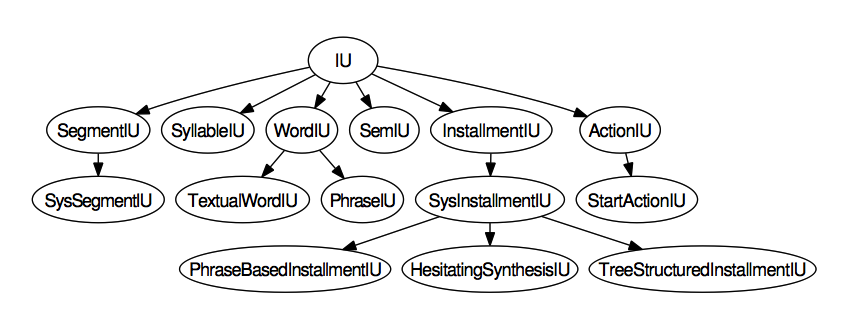
\includegraphics[width=1.0\textwidth]{images/IUs.png}
 \caption{ An excerpt of INproTk built-in type hierarchy \parencite
 {baumann2013:phd}}
  \label{fig:IUs}
\end {figure}
Processing of IUs is guarantied by IU modules. IU
modules consist of left buffer, right buffer and processors.  INproTK Different IUs
modules are interconnected with each other, forming a pipeline of IU modules \parencite {baumann2013:phd}. A typical
communication between two IU modules is shown in the figure \ref{fig:IUs}.
\begin{figure}[htbp]
  \centering
    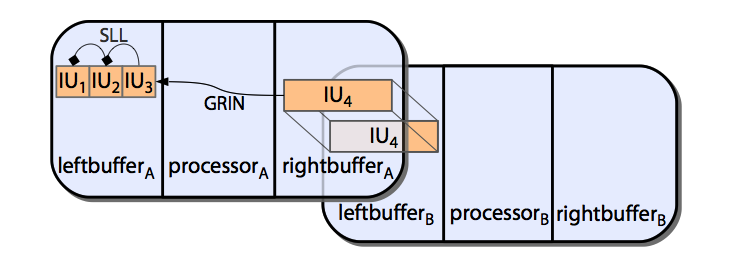
\includegraphics[width=1.0\textwidth]{images/iuandbuffer.png}
 \caption{ Incremental Modules and their intercommunication via left-right
 buffers \parencite {baumann2013:phd}}
  \label{fig:IUs}
\end {figure}
\section {INproTK IU Modules in Recognizer Architecture}
\subsection  {Google IU Module}
GoogleASR is a source IU module in InproTK, which listens to the
results coming from Google's  downstream connection in JavaScript Object Notation (JSON) format and
passes results to its listeners by updating the current hypotheses and providing
info about the hypotheses time (hypotheses start and end times).
 \begin{figure}[htbp]
  \centering
   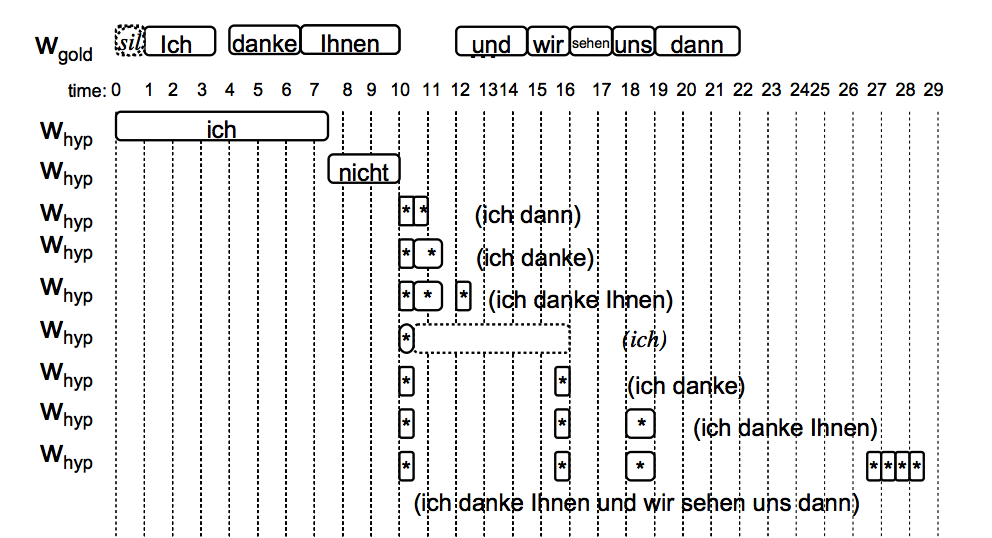
\includegraphics[width=0.9\textwidth]{images/google_output.png}
  \caption{Incremental output of Google ASR with existing timing}
  \label{fig:google_ouput}
\end{figure}

Timing, implemented in Google ASR, has nothing to do with true alignment.
With the help of this information  it is only possible to calculate the
timeliness: FO as well as FD.  Manual reconstruction of alignment from
timeliness is problematic as timeliness does not preserve any information about word
duration. 

For example, in the figure  \ref {fig:google_ouput} the first hypotheses (word
``ich) equals 0 and end times equals about 7.5 time slots, whereas the borders of the word
``ich'' are between 1 and 3.5 time slot. In addition, in case of Google we are dealing with additional output delay,
resulted from network latency, which can be slightly variable approximately
between 10 and 200 ms depending on the network configuration. Google has
processed the file till the end of the word ``ich'' by the time 3.5, after some internal Google offset, the output was made.
It is assumed, that Google offset reflects the problem of stability of the
the output and latency \parencite {mcgrawgrauenstein2012}. Finally, Google ASR returned this result after 
network delay.  
 \begin{figure}[htbp]
  \centering
   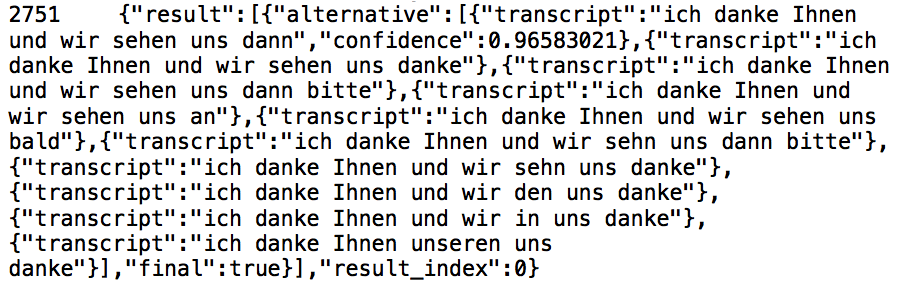
\includegraphics[width=1\textwidth]{images/json_extr.png}
    \caption{JSON file example}
      \label{fig:json_ouput}
\end{figure}
\subsection {Sphinx ASR Module and Label Writer in INproTK}
Sphinx ASR in INproTk is IU module that receives results from Sphinx-4
recognizer, transforms them to IUs of recognized words and sends them
to Label writer IU via left-right buffer configuration.   Label writer in its turn
is responsible for output of the recognition results and  their timing
information in the console. Apart from that Label writer  offers a configurable
option to save the recognition and timing results to a file. An extract of such
file is shown in the following figure. 

\section {Architecture Overview of the Google-Sphinx Recognizer}
Sphinx-Google architecture includes Sphinx-4 frontend, dictionary,
language model and acoustic model, decoder with search graph, forced-alignment
module, Sphinx control thread, synchronous blocking queue and InproTK IUs:
Google ASR, Sphinx ASR and label writer.  (see figure \ref {fig:arch}).
\begin{figure}[htbp]
  \centering
    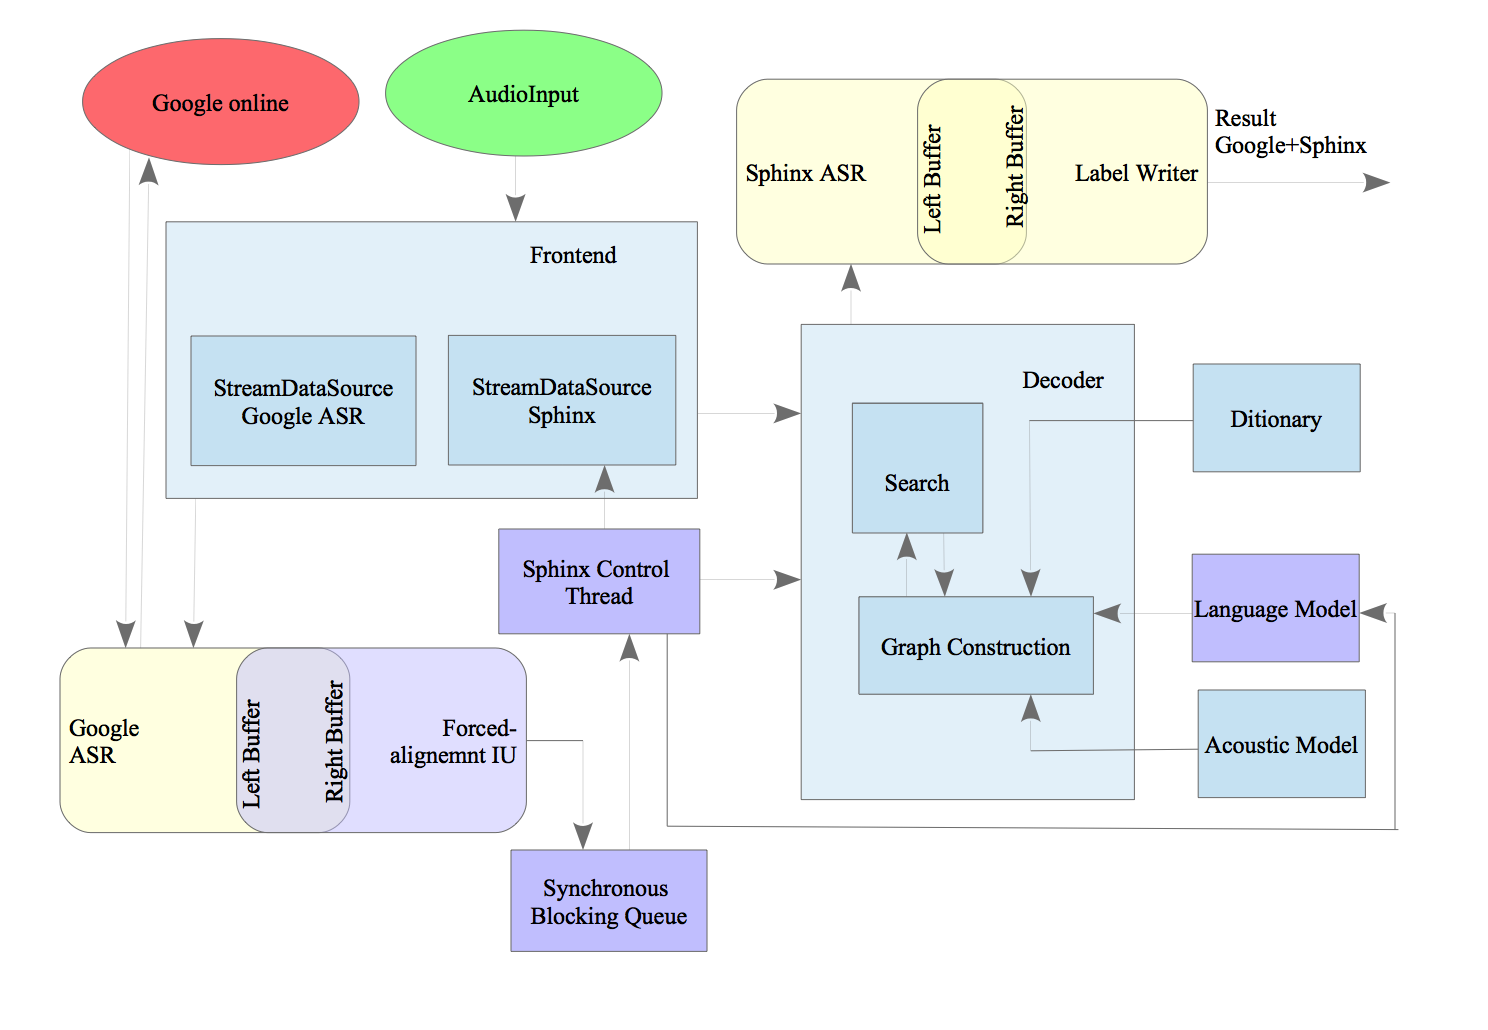
\includegraphics[width=1\textwidth]{images/architecture.png}
 \caption{Implementation Overview}
  \label{fig:arch}
\end {figure} 
%\subsection {Frontend}

As an audio input both Google ASR and Sphinx receive the same audio input.
Input stream of Google ASR is set only once, whereas the length of
the stream is equal to the whole audio. By contrast, the Sphinx input stream is
updated every time, Google ASR returns new hypothesis.  


GoogleASR listens to JSON results coming from online Google, running
in incremental mode, and passes result to forced-alignment IU. Google ASR result
is transferred to forced-alignment IU via standard IU left-right buffer. Google
ASR result contains hypothesis, and the start and end times, computed by Google
ASR for every hypothesis. 

Forced-alignment IU puts every incremental Google result into synchronous
blocking queue. Sphinx control thread takes the last Google hypothesis from the
synchronous blocking queue and starts Sphinx decoding. Sphinx control thread
updates language model, resetting text for alignment. As soon as the grammar of
the language model is changed, search graph of the decoder module is rebuild
anew. 


\section {Forced-alignment of Google Incremental Results with Google-Sphinx
Recognizer}

Every time the new hypothesis is taken from the queue Sphinx input stream  is
also reset. Analyses of Google JSON files, containing the hypotheses times of Google, show
that this time can be used to calculate the length of the input stream to be
updated. In the GoogleASR INproTK module output  (compare  \ref
{fig:google_ouput}) Google hypotheses time equals the end times of the word IU,
put in the left buffer. 

In the example \ref {fig:google_ouput}) the first hypotheses
``ich'' came from Google at 750 ms. By this time in audio the words ``ich danke
I\ldots'' already pronounced. If we substract network latency  
from the hypotheses time, than we know that that Google was ready with its
hypotheses several dozens milliseconds earlier.  In the case when latency is
equals 100 ms, that is 650 ms. However, 650 ms is still far from the true end
of the word ``ich'' in audio (350 ms). This difference of 300 ms is actually the
latency time Google needs to come to confident result, before it produce the
output. Under this consideration the following assumption is made: $Google
hypotheses time>=hypotheses end im audio + Google offset + network latency$.
With the first output Google waits 650 ms, the next outputs come 
after 0 to 850 ms relative to the previous output. 

In order to get correct alignment from Sphinx for  first Google result ``ich''
it is enough to restart Sphinx with the grammar, containing the word ``ich''
and piece of audio between 350 ms and 650 ms.  Alignment will also function  if
the whole input stream is reseted with every new hypotheses. However, with such
approach the processing time will grow quadratically (?) and the quality of
alignment will decrease. So the more accurate file length  matches the
transcription the better are the alignment results. 

\subsection {Forced-alignment mode of Sphinx+Google recognizer}

Sphinx-4 in its standard implementation is able to do either alignment or
recognition. Sphinx-4 Linguist example configuration, required for alignment, is
shown in the figure \ref{fig:conf_al}. As it is seen from the example in the
Sphinx+Google recognizer uses dynamic flat linguist and aligner grammar. 

\begin{figure}[htbp]
  \centering 
 
 \lstdefinestyle{nonumbers} 
{numbers=none}  
\lstset{language=XML} 
\lstset{ 
  backgroundcolor=\color{white},   % choose the background color; you must add \usepackage{color} or \usepackage{xcolor}
  basicstyle=\footnotesize,frame=single }  
%\begin{lstlisting}[frame=single]
 %backgroundcolor=\color{white}, 
 %\begin{lstlisting}  
\begin{lstlisting}[style=nonumbers]

...
<component name="linguistFA" type="edu.cmu.sphinx.linguist.dflat.DynamicFlatLinguist">  
        <property name="logMath" value="logMath"/>
       <property name="grammar" value="forcedAligner"/>   
        <property name="acousticModel" value="acousticModel"/>
        <property name="wordInsertionProbability" value="${wordInsertionProbability}"/>
        <property name="silenceInsertionProbability" value="${silenceInsertionProbability}"/>
        <property name="languageWeight" value="${languageWeight}"/>
        <property name="unitManager" value="unitManager"/>
    </component>

...
\end{lstlisting}
 \caption{Extract from configuration file for Google-Sphinx Recognizer in
 alignment mode}
  \label{fig:conf_al}
\end {figure}

Timing results of Sphinx, started after Google, are shown in the figure below
(\ref{fig:conf_al_timing}):
\begin{figure}[htbp]
  \centering
    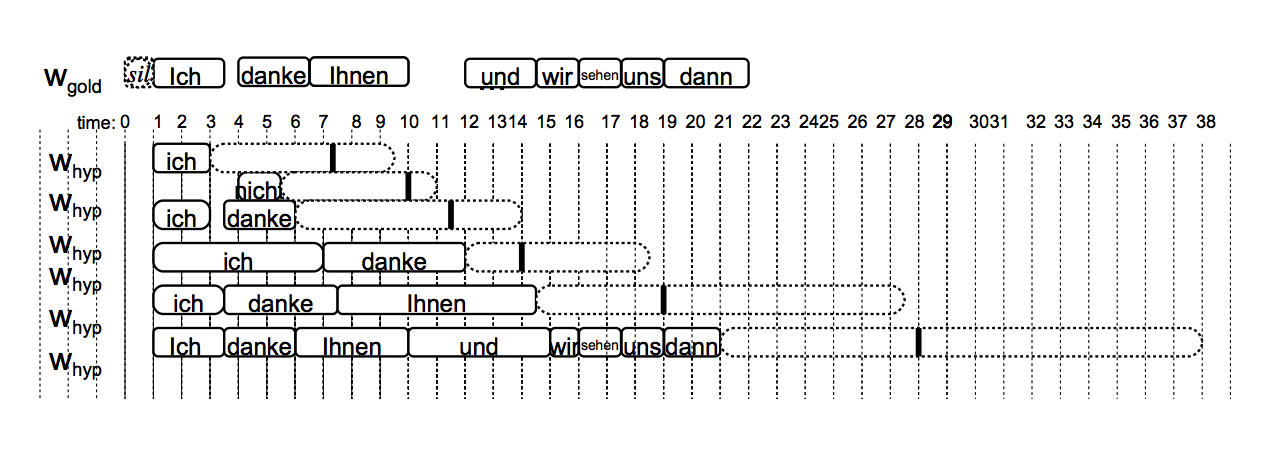
\includegraphics[width=1.0\textwidth]{images/google_sphinx_output_al.png}
 \caption{Google+Sphinx output with improvement timing. Vertical lines shows
 the time, by which Google was ready with the corresponding hypotheses.
 Right borders of the dotted boxes shows at what point of time Sphinx was ready
 with its alignment.}
  \label{fig:conf_al_timing}
\end {figure}

Comparison of visualization results with the corresponding Google
output ((\ref{fig:google_ouput}) demonstrates qualitative timing improvement in terms
of error rate, whereas the WER remains unchanged, as the output contains the
same result as that of Google alone. The number of hypotheses is smaller,
because Sphinx gets incremental results for processing only when
forced-alignment of one result is finished.  If during Sphinx processing time
Google produce additional hypotheses, this hypotheses are skipped and only the
last one is taken for new processing. 

However, an obvious disadvantage of this alignment approach is additional
latency produced by Sphinx during alignment.
Alignment task, where the search path is known and defined is less time
consuming as recognizing, demands nevertheless computation time.  Computation
time depends on the processing power. If the Sphinx processing time could have
been neglected, than we get an model of Google+Sphinx recognizer,
comparable to Google in WERs and having an improved timing.

\subsection {Forced-alignment and recognition mode  of Sphinx+Google recognizer}

In the second approach Sphinx returns not only alignment result, based on Google
ASR, but continues with recognition, while waiting for the new Google incremental result. 
This approach solves several tasks. First, we get more precise alignment  in
case of excessive input stream. Moreover, excessive input stream is
even desirable as only additional frames guarantees recognition start after
alignment is finished. Second, Sphinx produce some results with better
timeliness, if it has finished alignment and is waiting for new Google
hypotheses. Third, it possible to use the Google result to manipulate the search
path in search graph of Sphinx and theoretically change to a path proposed by
Google, if this path exist. 

Configuration of Sphinx+Google recognizer in alignment and recognition mode
uses dynamic flat linguist, because of the  advantages, described in the chapter
\label{ref:sphinx}. As a grammars the following types were tested: JSGF grammar
and n-gram Gram, based on default language model.  However, by contrast to standard Grammar
implementation in Sphinx these grammars are combined with alignment grammar in
their implementation.


\begin{figure}[htbp]
  \centering 
 
 \lstdefinestyle{nonumbers} 
{numbers=none}  
\lstset{language=XML} 
\lstset{ 
  backgroundcolor=\color{white},   % choose the background color; you must add \usepackage{color} or \usepackage{xcolor}
  basicstyle=\footnotesize,frame=single }  
%\begin{lstlisting}[frame=single]
 %backgroundcolor=\color{white}, 
 %\begin{lstlisting}  
\begin{lstlisting}[style=nonumbers]

...

      <component name="linguistFA"type="edu.cmu.sphinx.linguist.dflat.DynamicFlatLinguist"> 
      <property name="logMath" value="logMath"/>
        <property name="grammar" value="ngramGrammar"/> 
        <!--  <property name="grammar" value="myjsgfGrammar"/>--> 
        <property name="acousticModel" value="acousticModel"/>
        <property name="wordInsertionProbability" value="${wordInsertionProbability}"/>
        <property name="silenceInsertionProbability" value="${silenceInsertionProbability}"/>
        <property name="languageWeight" value="${languageWeight}"/>
        <property name="unitManager" value="unitManager"/>
    </component>

...
\end{lstlisting}t 
 \caption{Extract from configuration file for Google-Sphinx Recognizer in
 alignment and recognition mode}
  \label{fig:conf_al_rec}
\end {figure}


\ldots How the grammar are combined write here in some more details with example
probably. 

\subsection {Alignment +Recognition with JSGF Grammar}
To demonstrate that alignment and recognition are able to be combined any
type of JSGF grammar can be used. However, as JSGF grammar describe 
relative small command languages, we used a phone loop grammar in JSGF format,
suitable for more universal tasks.

An example of such grammar is shown in the figure   \ref{fig:phone_loop}

\begin{figure}[htbp]
 % \centering 
%  \lstset{
%   literate={@}{{\"u}}1
% }
%  \lstdefinestyle{nonumbers} 
%  {numbers=none} 
%  
%  
% %\begin{center}
% %\begin{lstlisting}[style=nonumbers]

grammar phones;

public <phones> = \begin{IPA}(2: | 6 | 9 | @ | C | E | E: | I | N | O | OY | Q |
S | SIL | U | Y | Z  | a | a: | aI | aU | b | d | e |  e: | f | g |h | i | i: |
j | k | l | m | n | o | o: | p| r | s |  t | u | u: | v | x | y: | z
)*;\end{IPA}


%\end{center}
%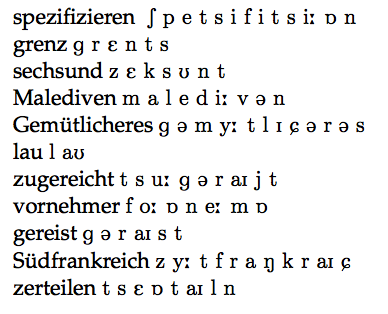
\includegraphics[width=0.5\textwidth]{images/dic.png}
 \caption{An extract from the dictionary file.}
  \label{fig:phone_loop}
\end {figure}

Described phone-loop grammar is prototypical and uses no weights. Result of the
recognition of audio with transcription ``eins zwei drei vier'', using the
phone-loop grammar   \ref{fig:phone_loop} are shown in the figure
\ref{fig:phone_loop_res}.


\begin{figure}[htbp]
 \centering 

  \lstdefinestyle{nonumbers} 
  {numbers=none} 
  
\begin{center}
\begin{lstlisting}[style=nonumbers]


0.000	0.680	ein
0.430	1.030	zwei
0.720	0.760	<sil>
0.860	0.890	<sil>
0.890	0.920	<sil>
0.920	1.010	c
1.010	1.070	i
1.070	1.120	6
1.120	1.200	i
1.200	1.310	e
1.310	1.420	sil
1.420	1.610	e
1.610	1.670	l
1.670	1.720	i
1.720	1.990	l
1.990	2.040	p
2.040	2.140	p
2.140	2.340	i
2.340	2.490	e
2.490	2.580	6
2.580	2.640	r
2.640	2.710	sil
2.710	2.780	<sil>


\end{lstlisting}
\end{center}
%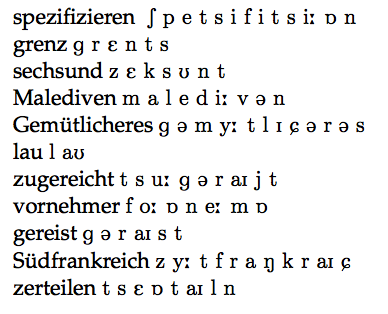
\includegraphics[width=0.5\textwidth]{images/dic.png}
 \caption{Alignment + Recognition result, using combined grammar, based on
 fixed input ``eins zwei'' and phone-loop JSGF grammar for the audio, having
 transcription ``eins zwei drei vier'' (\ref{fig:phone_loop_res})}.
 
  \label{fig:phone_loop_res}
\end {figure}


\subsection {Alignment +Recognition with N-Gram Grammar}



%\section {Forced-alignment mode versus }
\section {Timeliness Improvement}




% The initialisation and implementation of the SearchGraph is realised by
% Sphinx-4. The choice and alternation of the path in
% the SearchGraph depends on the Google incremental hypotheses. 
% When the new Google hypotheses differs from the present hypotheses in the
% SearchGraph, the SearchGraph is reseted and the hypotheses path is
% corrected.  Timeliness improvement is supposed to be achieved by faster results
% produced by Sphinx, whereas the path in the Sphinx SearchGraph is predetermined
% by Google incremental result. The last means that we get the same final results
% for Google and Google + Sphinx, but timeliness of Google + Sphinx
%is expected to be improved. 
\section {Search Module of Google-Sphinx Recognizer}
\subsection {Decoder configuration}
\subsection {Search Modification}